% (c) Gerard Baecker
\documentclass[fleqn,a4paper,12pt]{article}
\usepackage{geometry}
\geometry{left=30mm, right=40mm, bottom=30mm}
  \usepackage[german]{babel}
  \usepackage[utf8]{inputenc}
  \usepackage{amsmath}    % Mathematische Symbole
  \usepackage{amssymb}     % Nochmehr mathematische Symbole
  \usepackage{dsfont}      % Schriftsatz fuer Zahlenmengensymbole
  %\usepackage{verbatim}   % erweiterte Verbatim-Umgebung
  \usepackage{alltt}       % Quasi-Verbatim-Umgebung
  \usepackage{fancyhdr}    % Eigene Kopfzeilen
  \usepackage{graphicx}    % Zum Einbinden von Grafiken
  % Einbinden einer eps-Grafik geht so: includegraphics{path}
  \usepackage{wrapfig}
  \usepackage{lscape}
  \usepackage{rotating}
  \usepackage{epstopdf}
  
  % Seitenraender
  \addtolength{\voffset}{-2cm}
  \addtolength{\textheight}{0cm}
  \addtolength{\hoffset}{0cm}
  \addtolength{\textwidth}{2cm}
  \addtolength{\headheight}{2cm} % fuer jeden Strichkode einen Zentimeter
  
  % Skalierung der Grafiken
  \setlength{\unitlength}{1cm}
  
  \pagestyle{fancy}            % Eigene Kopfzeilen verwenden
  \frenchspacing               % Kein Extrafreiraum nach Satzzeichen
  \setlength{\parindent}{0pt}  % Neue Absaetze nicht einruecken
  %\sloppy                     % Schlampige Absatzformatierung
  \fussy                       % Penible Absatzformatierung
  \linespread{1.5}             % Zeilenabstand
  
  % Font fuer Code 39
  \font\xlix=wlc39 scaled 1200
  \newcommand\barcode[1]{{\xlix@#1@}}
  
  % Name, Matrikelnummer, Barcode
  \newcommand\student[2]{
    \mbox{\scriptsize
    \begin{tabular}{@{}l@{}r@{}}
      \multicolumn{2}{@{}r@{}}{\barcode{#2}}\\
      #1&#2\\
    \end{tabular}}}

%andere Definitionen
\newcommand{\R}{{\mathbb R}}
\newcommand{\N}{{\mathbb N}}
\newcommand{\Z}{{\mathbb Z}}
\newcommand{\Q}{{\mathbb Q}}
\newcommand{\C}{{\mathbb C}}
\newcommand{\F}{\mathcal{F}}
\newcommand{\less}{\setminus}
\newcommand{\inv}{{}^{-1}}
\newcommand{\Land}{\bigwedge}
\newcommand{\Lor}{\bigvee}

  % Kopfzeile
  \lhead{
    \small
    \textsc{Grundlagen der Signalverarbeitung \\
      WS 2017/2018 \\
      \"Ubung (\today)}
    \vfill}
  \rhead{
    \begin{tabular}[b]{@{}rr@{}}
      \student{Philipp Badenhoop}{572693} &
      \student{Steven Lange}{568733} \\
      \student{Pascal Jochmann}{575056} &
      \student{Kevin Trogant}{572451}
    \end{tabular}}
  
  \begin{document}
  "Ubungsaufgabe 7: \newline
  Aus der Dichtefunktion $p(x) = \lambda e^{-\lambda x}$, $x \geq 0$ ergibt sich die Verteilungsfunktion: \[F(x) = \int p(x) dx = -e^{-\lambda x} + C\]
  Für kontinuierliche Zufallsgrößen ergibt sich der gesuchte \textit{Median} $x_{med}$ folgendermaßen:
  \begin{align*}
      \int_{-\infty}^{x_{med}} p(x) dx &= \frac{1}{2} \\
      \Leftrightarrow \quad \int_0^{x_{med}} p(x) dx &= \frac{1}{2} \quad \text{Da }  p(x) = 0 \text{ für } x < 0 \\
      \Leftrightarrow \left[ -e^{-\lambda x} + C \right]_{0}^{x_{med}} &= \frac{1}{2} \\
      \text{Wähle } \lambda = \frac{1}{2} \\
      \Rightarrow \quad -e^{-\frac{1}{2}x_{med}} + 1 &= \frac{1}{2} \\
      \Rightarrow x_{med} = -2 \cdot \ln \frac{1}{2}
  \end{align*}
  Der Erwartungswert ergibt sich aus \[E(X) = \int_{-\infty}^{+\infty} x \cdot  p(x) dx\] \\
  Lösen des Integrals ergibt dann $E(X) = 2$. \\
  Die Varianz ergibt sich aus \[\textit{Var}(X) = \int_{-\infty}^{+\infty} ( x - E(X) )^2 \cdot p(x) dx\]
  Lösen des Integrals ergibt dann $\textit{Var}(X) = 4$.
  \begin{figure}
      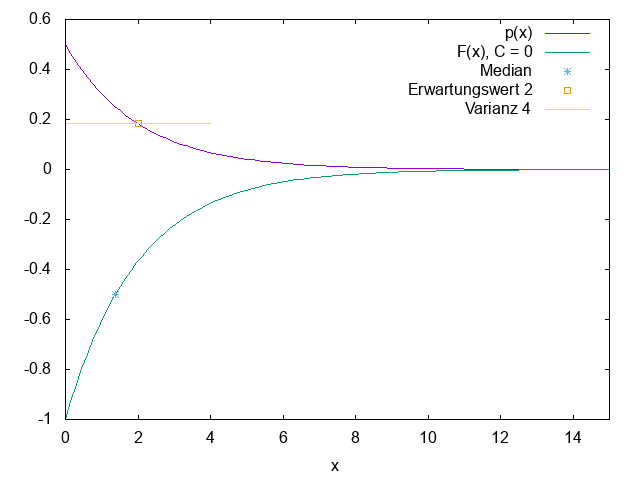
\includegraphics[width=1.0\textwidth]{sv0_7.png}
      \caption{(7) Darstellung der gegebenen Dichtefunktion und einiger Kenngrößen}
  \end{figure}
  \newpage
	"Ubungsaufgabe 8: \newline
	Sei folgendes Tertiärsignal gegeben:\\
	\begin{tabular}{|c|p{0.6cm}|p{0.35cm}|p{0.35cm}|p{0.35cm}|p{0.35cm}|p{0.35cm}|p{0.35cm}|p{0.35cm}|p{0.35cm}|p{0.35cm}|p{0.5cm}|p{0.15cm}|p{0.2cm}|p{0.2cm}|p{0.2cm}|p{0.2cm}|p{0.2cm}|p{0.2cm}|p{0.2cm}|p{0.2cm}|p{0.4cm}|}
		\hline
		Messwert	& -10 & -9 & -8 & -7 & -6 & -5 & -4 & -3 & -2 & -1 & 0 & 1 & 2 & 3 & 4 & 5 & 6 & 7 & 8 & 9 & 10\\
		\hline
		Anzahl		& 1 & 2 & 3 & 4 & 50 & 6 & 5 & 4 & 3 & 2 & 228 & 2 & 3 & 4 & 5 & 6 & 50 & 4 & 3 & 2 & 1\\
		\hline
	\end{tabular}\\
	\\
	Aus den 388 Daten der Zufallsvariable $X$ lassen sich nun folgende Werte entnehmen:
	\begin{align*}
	m_1 = E[X]				=& \int_\Z x\rho(x) \mu(dx) = \sum_{x=-10}^{10} x\rho(x)= \frac{0}{388} = 0\\
	z_2 = Var(X) = \sigma^2	=& E\left[\left(X-E[X]\right)^2\right] = E\left[X^2 - 2E[X]X + E[X]^2\right]\\
	=& E\left[X^2\right] - E\left[2E[X]X\right] + E\left[E[X]^2\right]\\
	=& E\left[X^2\right] - 2E[X]E\left[X\right] + E[X]^2 E\left[1\right]\\
	=& E\left[X^2\right] - 2E[X]^2 + E[X]^2 \cdot 1 = E\left[X^2\right] - E[X]^2\\
	=& \int_\Z x^2\rho(x) \mu(dx) - E[X]^2 = \sum_{x=-10}^{10} x^2\rho(x) - 0^2\\
	=& \frac{5460}{388} \approx 14,07\\
	\sqrt{z_2} = \sigma		\approx& 3,75\\
	\end{align*}
	Wobei, wie aus Stochastik I bekannt, der Erwartungswert von $X$ $E[X]$ ein lineares Funktional, $\mu$ das kanonische Zählmaß und $\rho(x)$ die relative Häufigkeit von $x$ ist\\
	\\
	Da $m_1 = E[X] = 0$ gilt $\forall i\in\N:m_i = z_i$\\
	$z_0 = \sum_{x=-10}^{10} \rho(x) = 1$ nach Definition.\\
	$z_1 = m_1 = 0$\\
	$z_2 \approx 14,07$\\
	$z_3 = \sum_{x=-10}^{10} x^3\rho(x) =  0$\\
	$z_4 = \sum_{x=-10}^{10} x^4\rho(x) \approx  593,91$\\
	\newpage
	\begin{figure}
		%\centering
		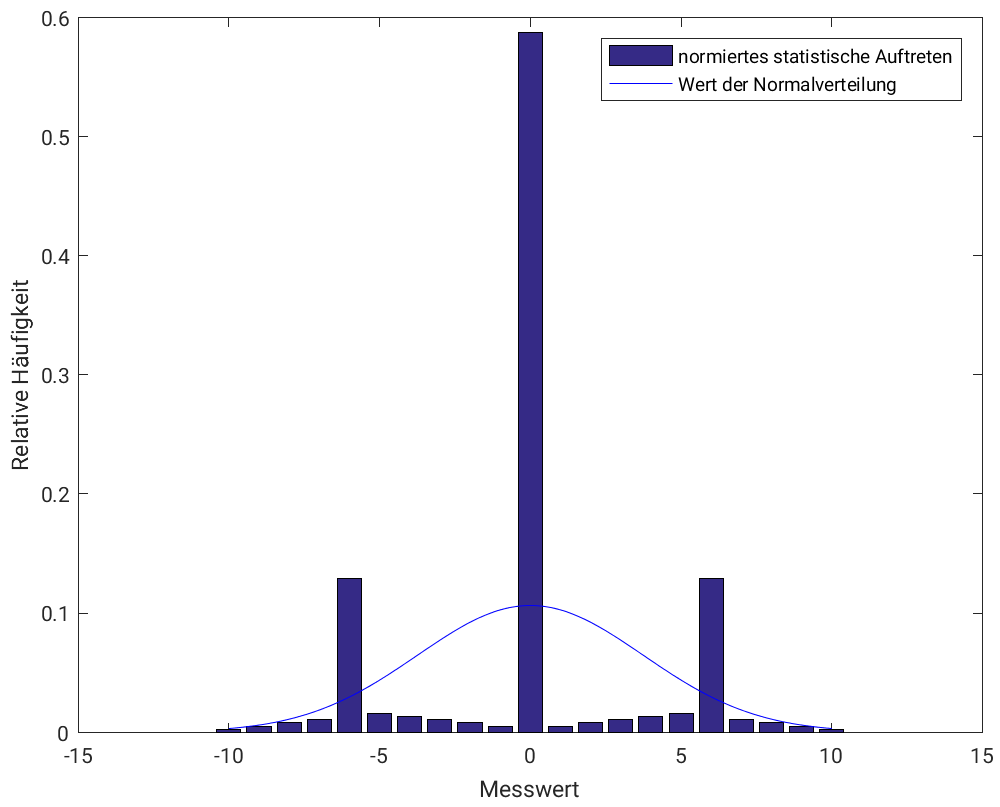
\includegraphics[scale = 0.9]{A8_Histogramm.png}
		\caption{Darstellung des Histogramms und der Glockenkurve}
	\end{figure}
	Mit der Formel $\mathfrak{Z}_k := \frac{z_k}{\sqrt{z_2^k}}$ ergibt sich:\\
	$\mathfrak{Z}_0 := \frac{z_0}{\sqrt{z_2^0}} = \frac{1}{1} = 1$\\
	$\mathfrak{Z}_1 := \frac{z_1}{\sqrt{z_2^1}} = \frac{0}{\sigma} = 0$\\
	$\mathfrak{Z}_2 := \frac{z_2}{\sqrt{z_2^2}} = \frac{z_2}{z_2} = 1$\\
	$\mathfrak{Z}_3 := \frac{z_3}{\sqrt{z_2^3}} = \frac{0}{\sqrt{z_2^3}} = 0$\\
	$\mathfrak{Z}_4 := \frac{z_4}{\sqrt{z_2^4}} = \frac{z_4}{z_2^2} \approx \frac{593,91}{197,96} \approx 3,0$\\
	\\
	Nach den normierten Zentralmomenten hat das gegebene Ternärsignal die selbe Symmetrie und Wölbung wie die Glockenkurve.
  \newpage
  "Ubungsaufgabe 9: \newline
  \begin{sidewaysfigure}
      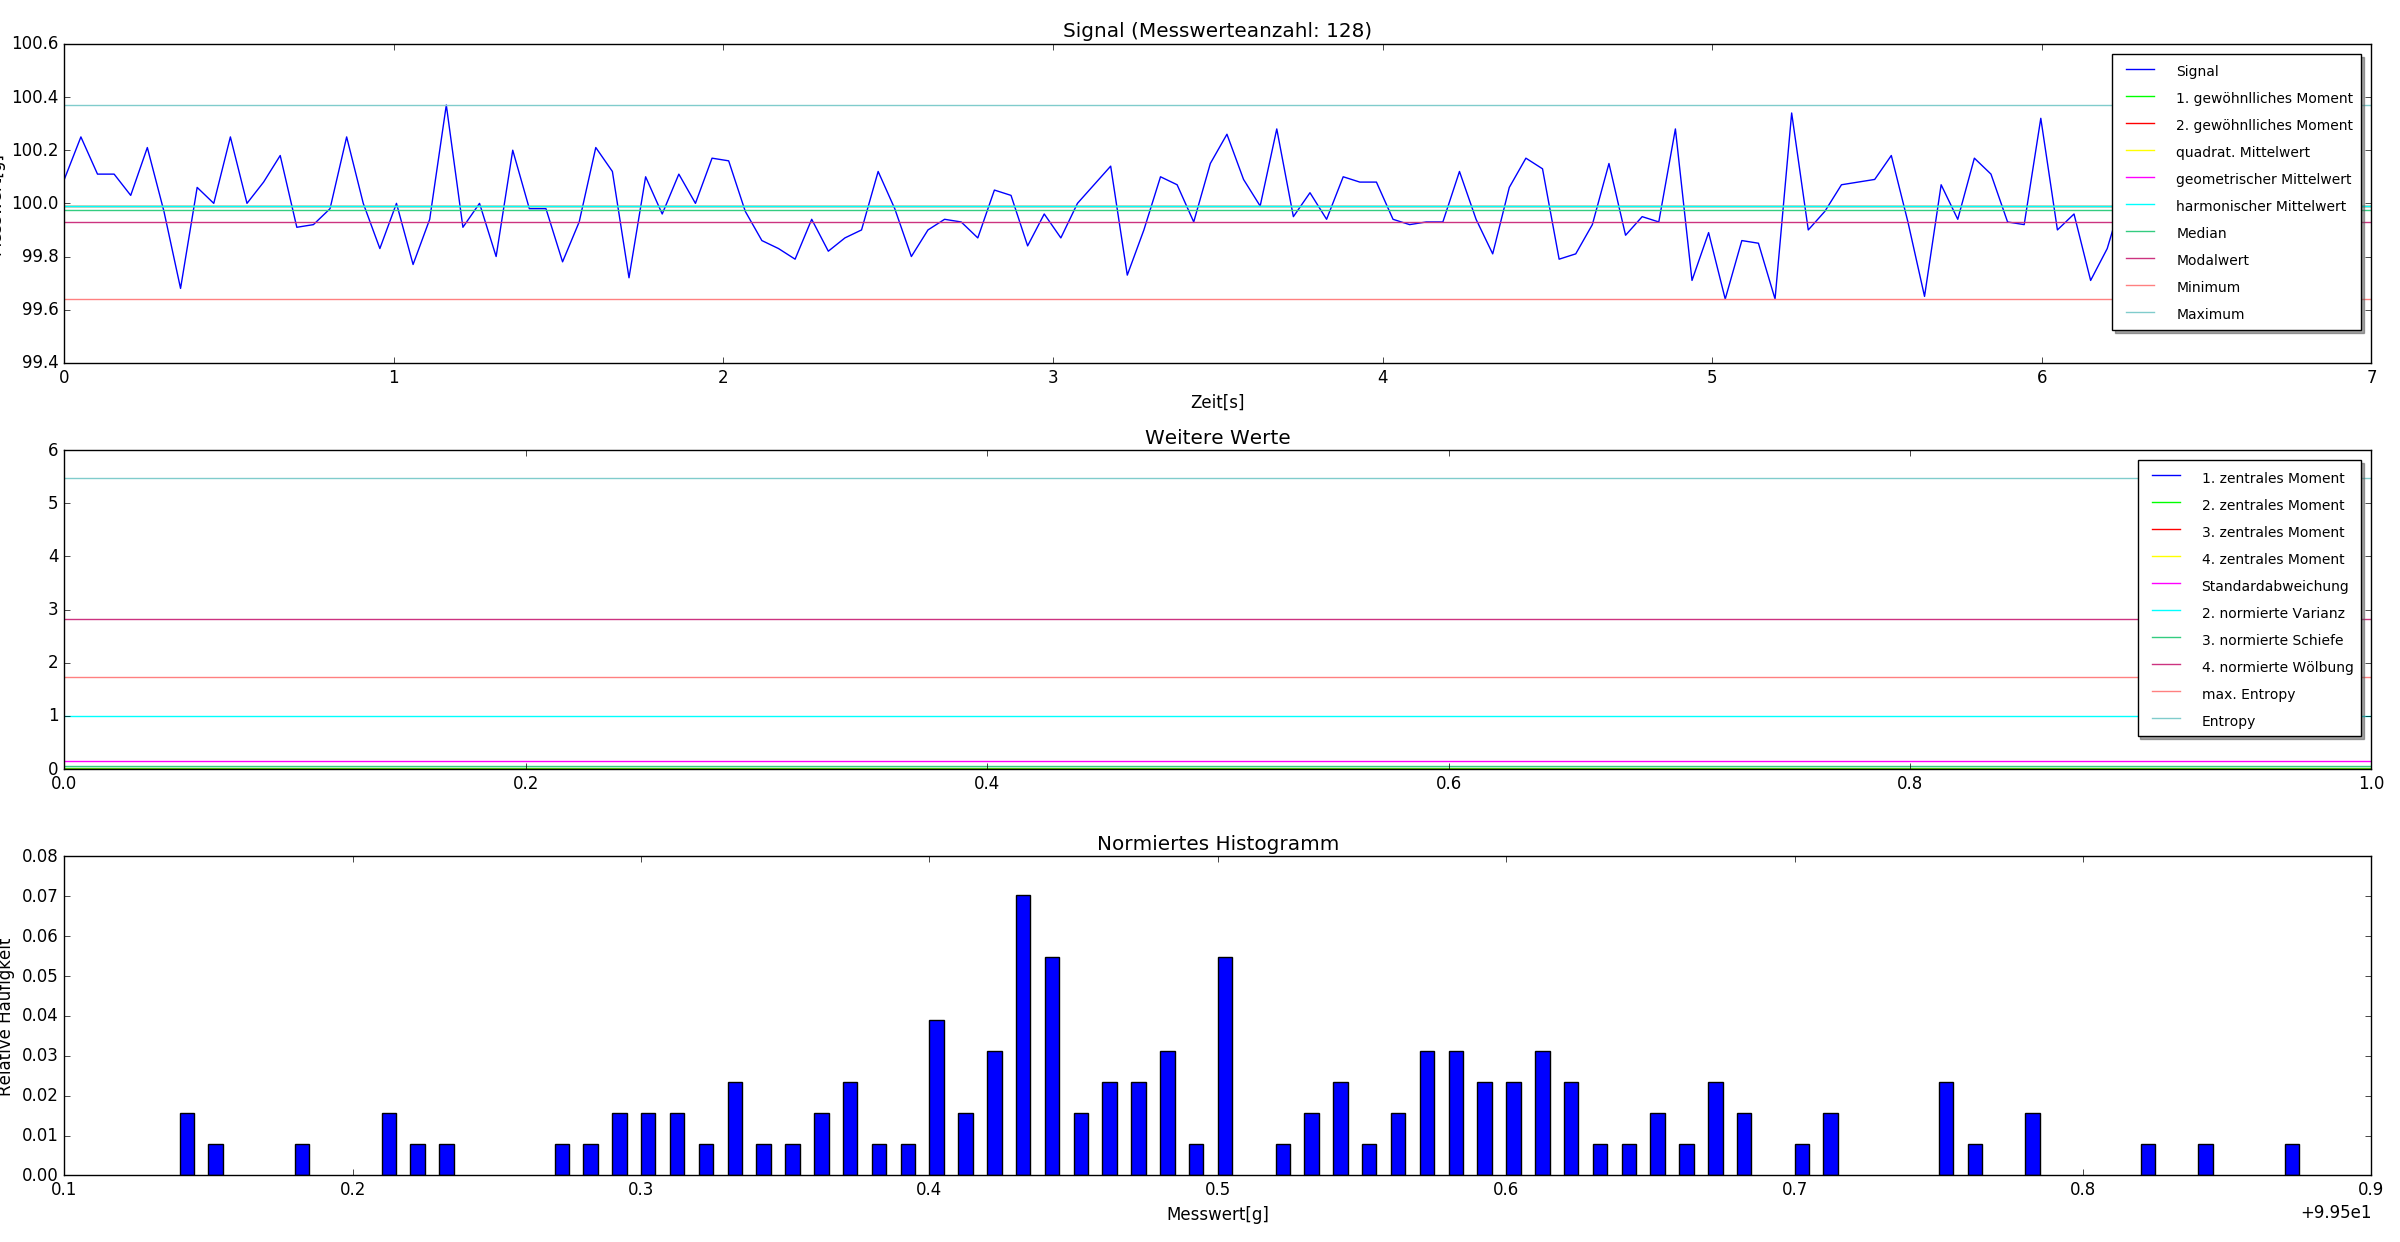
\includegraphics[width=1.0\textwidth]{a9_128.png}
      \caption{(9) Messreihe mit 128 Messwerten}
  \end{sidewaysfigure}
  \begin{sidewaysfigure}
    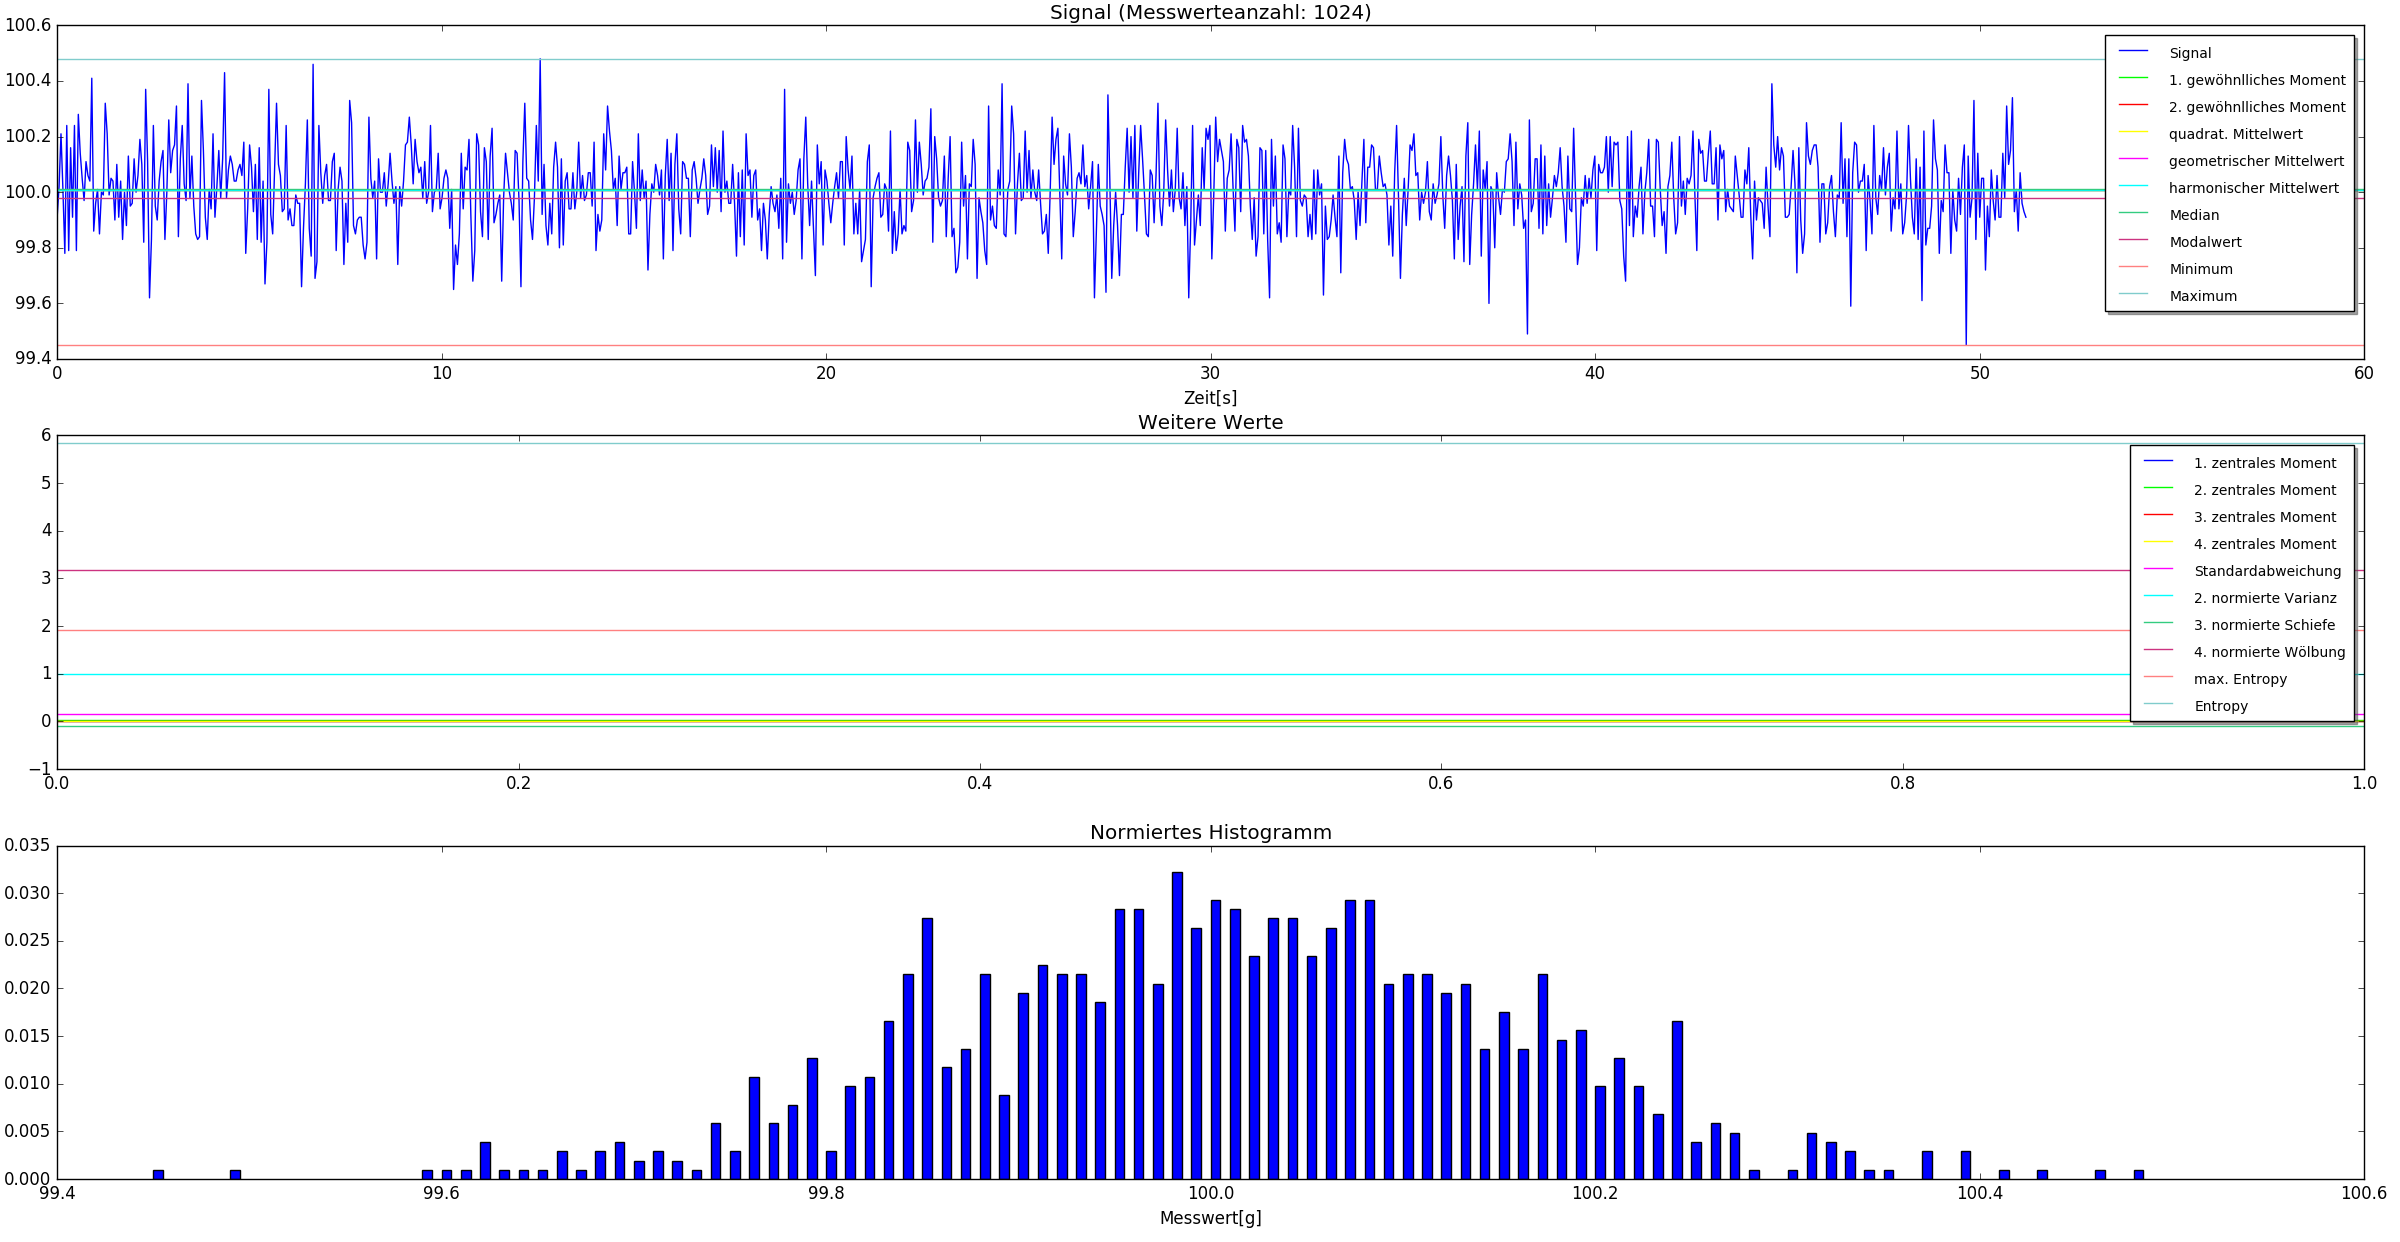
\includegraphics[width=1.0\textwidth]{a9_1024.png}
    \caption{(9) Messreihe mit 1024 Messwerten}
  \end{sidewaysfigure}
  Zur Messreihe mit 1024 Messwerten: \newline
  Mittelungleichung von Cauchy erfüllt: ja \newline
  Normalverteilt: ja \newline
  Interpretation Entropie: Der mittlere Informationsgehalt (Entropie) liegt mit $\approx 5.9$ relativ nah am maximalen Informationsgehalt $\approx 6.4$ (max. Entropie).
  Damit ist der Informationsgehalt eines Messwertes relativ groß. \newpage

  "Ubungsaufgabe 10: \newline
  \begin{sidewaysfigure}
    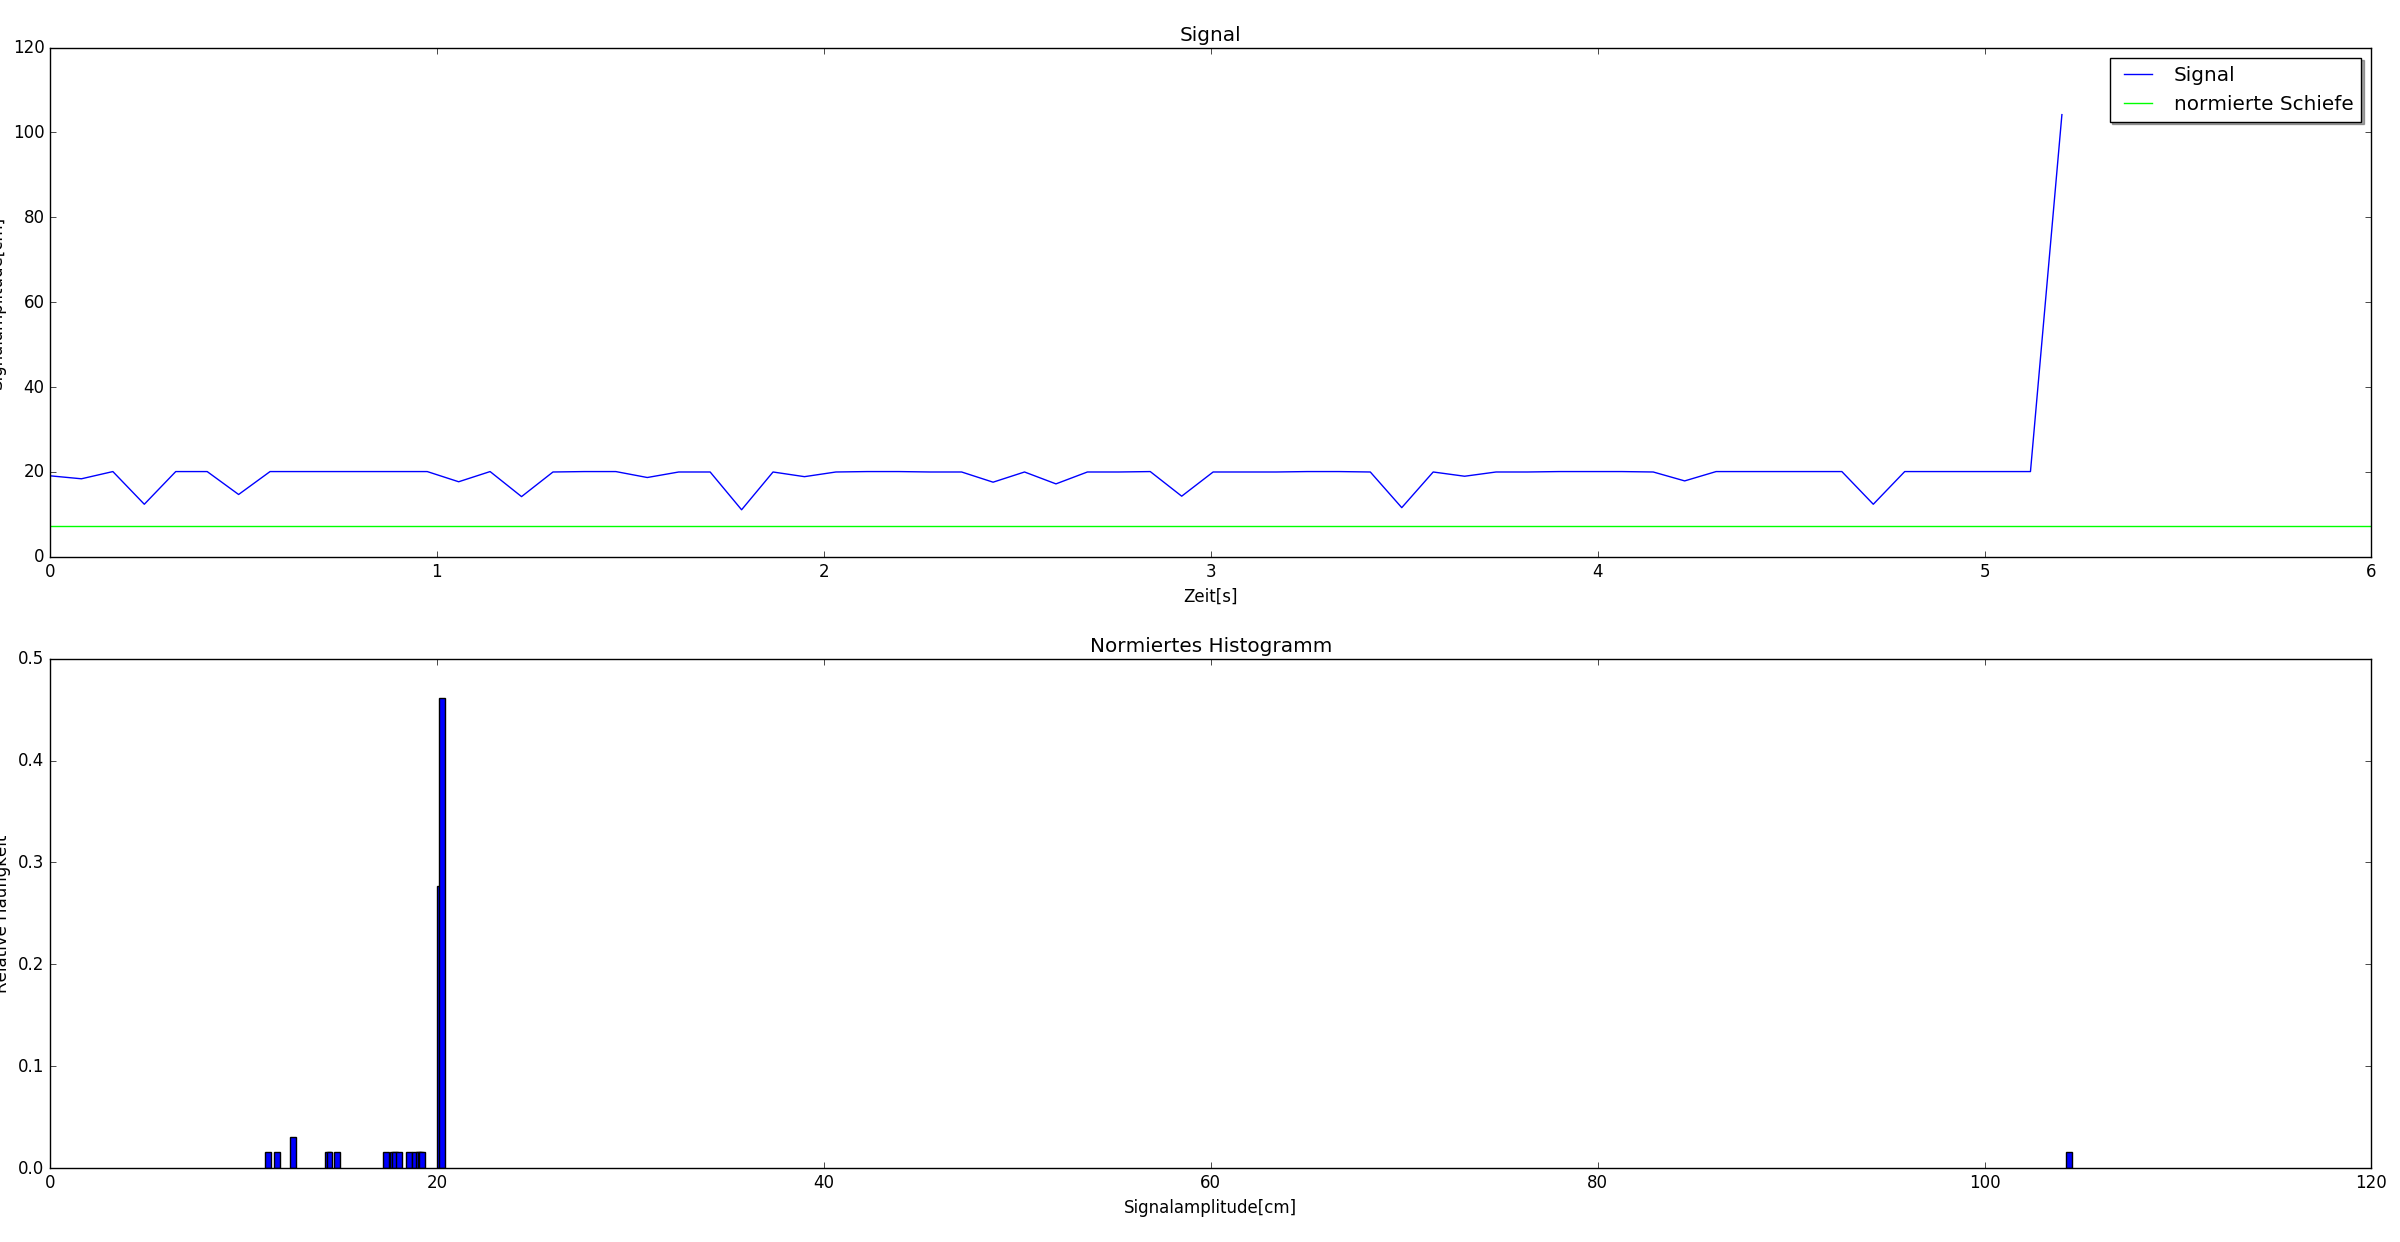
\includegraphics[width=1.0\textwidth]{a10.png}
    \caption{(10) Chaospendelprozess}
  \end{sidewaysfigure}
  Normierte Schiefe $\approx 7.32$ \newline
  Anmerkung: Hier scheint irgendetwas mit der Website schief zu laufen, da obwohl 128 Messwerte angefordert werden, nur 65 angezeigt werden.
  Außerdem sieht der Prozess nicht nach einem Chaospendel aus.
\newpage
  "Ubungsaufgabe 11:\newline

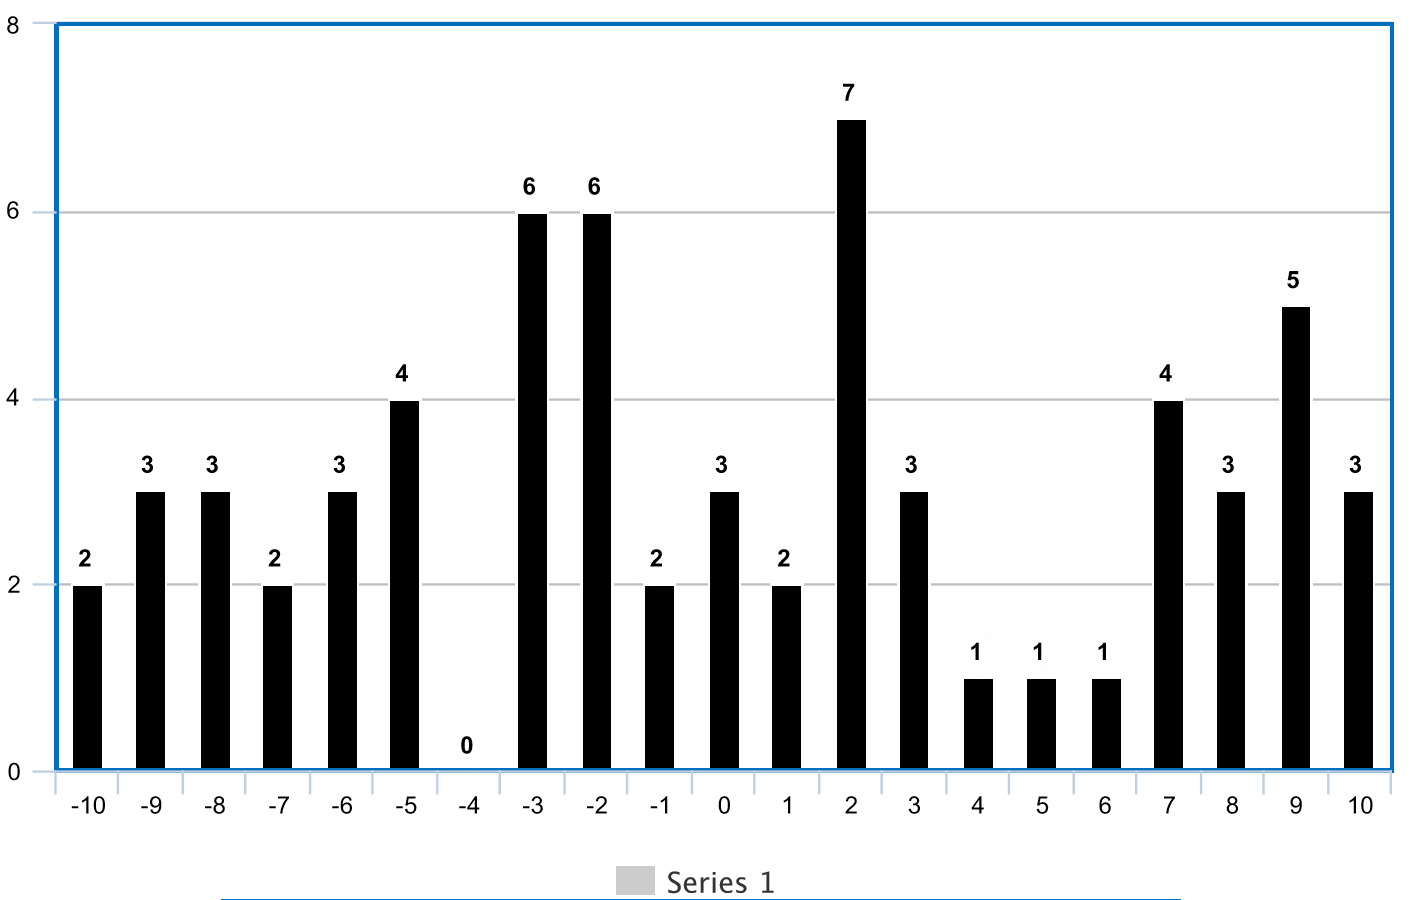
\includegraphics[scale=0.4]{H2}

a)Ganzes Signal:\\
$m_1 = 0,19		z_2 = 35$ \hspace{1cm}
Median = 0,	Modalwerte: -4 und 2

Signal in zwei H\"alften:\\
Erste H\"alfte:	\hspace{5cm}										Zweite H\"alfte:\\
$m_1 = 0,219$  $z_2 = 25$	\hspace{4cm}								$m_1 = -0,157$  $z_2 = 24$\\
\\
b)\\
Es K\"onnen 16 nicht \"uberlappende Episoden heraugeschnitten werden.
Episodemittelswertvektor: $m = \frac{1}{M}\sum_{i=0}^{M-1}e_i$\\
$m = (-2,94, 1,38, 1,25, 1,06)^T$\\
Keiner der Scharmittelwerte entspricht m1 $\rightarrow$ Signal ist weder station\"ar noch ergodisch.
\newpage
Kovarianzmatrix: $S = \frac{1}{M}\sum_{i=0}^{M-1}(e_i-m)(e_i-m)^T$\\
$
\begin{bmatrix}
21   & -6,3 & 1,4	 &  -1,8 \\
-6,3 & 44 	& -18	 &  -8 \\
1,4  & -18	& 29 	 & -4,3 \\
-1,8 & -8 	& -4,3	 &  34
\end{bmatrix}
$\\
Korrelationsmatrix $R_{u,v} = \frac{S_{u,v}}{\sqrt{S_{u,v} \sqrt{S_{u,v}}}}$
$
\begin{bmatrix}
1   & -0,21 & 0,06	 &  -0,07 \\
-0,21 & 1 	& -0,5	 &  -0,21 \\
0,06  & -0,5	& 1 	 & -0,14 \\
-0,07 & -0,21 	& -0,14	 &  1
\end{bmatrix}
$\\Die Werte abseits der Hauptdiagonale sind (im Betrag) klein, $\rightarrow$ das Signal ist zuf\"allig\\

\newpage

  "Ubungsaufgabe 12: \newline

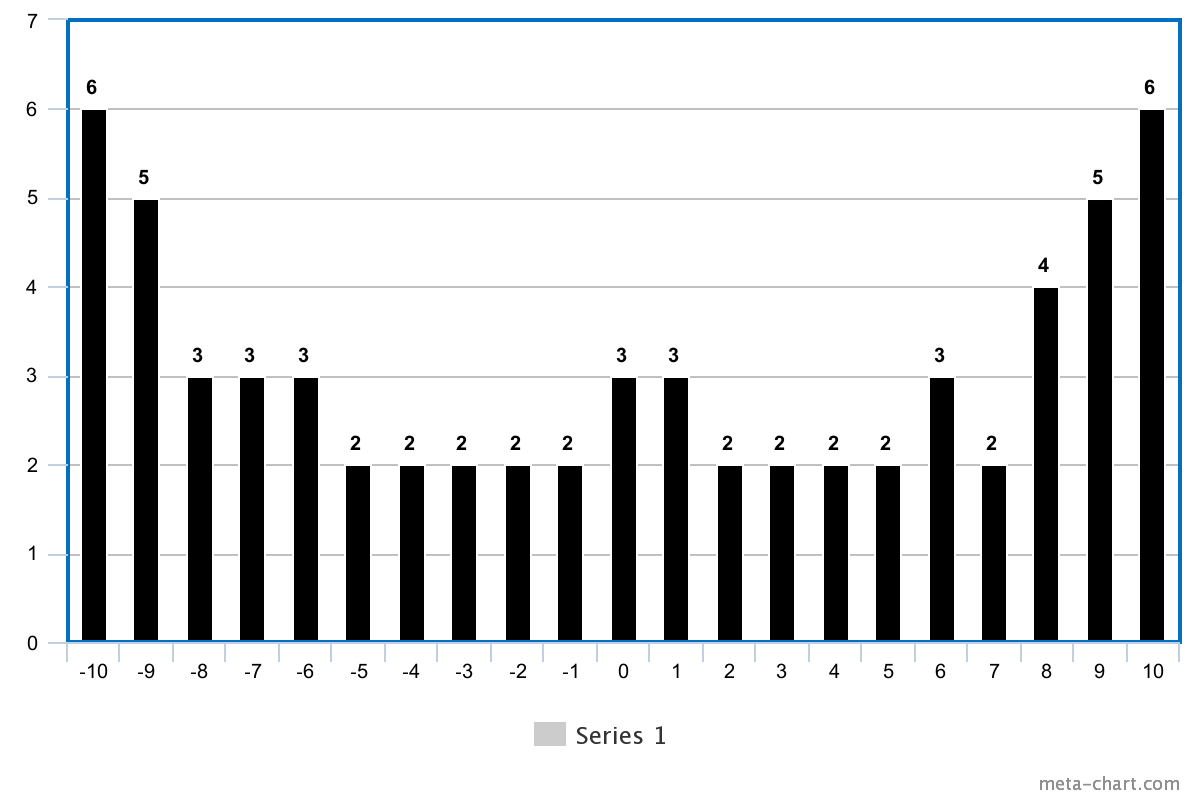
\includegraphics[scale=0.4]{H3}

a)Ganzes Signal:\\
$m_1 = 0,031		z_2 = 49$ \hspace{1cm}
Median = 0,	Modalwerte: $\pm $10

Signal in zwei H\"alften:\\
Erste H\"alfte:	\hspace{5cm}										Zweite H\"alfte:\\
$m_1 = 0,21875$  $z_2 = 25$	\hspace{4cm}								$m_1 = -0,15625$  $z_2 = 24$\\
\\
b)\\
Es K\"onnen 16 nicht \"uberlappende Episoden heraugeschnitten werden.
Episodemittelswertvektor: $m = \frac{1}{M}\sum_{i=0}^{M-1}e_i$\\
$m = (0, 0,063, 0, 0,063)^T$\\
Seine Scharmittelwerte sind \"ahnlich $m_1 \rightarrow$ Signal ist  station\"ar und ergodisch.
\newpage
Kovarianzmatrix: $S = \frac{1}{M}\sum_{i=0}^{M-1}(e_i-m)(e_i-m)^T$\\
$
\begin{bmatrix}
49   & 45 & 33	 &  16 \\
45 & 49 	& 45	 &  33 \\
33  & 45	& 48 	 & 45 \\
16 & 33	& 45	 &  49
\end{bmatrix}
$\\
Korrelationsmatrix $R_{u,v} = \frac{S_{u,v}}{\sqrt{S_{u,v} \sqrt{S_{u,v}}}}$
$
\begin{bmatrix}
1   & 0,91 & 0,67	 &  0,32 \\
0,91 & 1 	& 0,92	 &  0,68 \\
0,67 & 0,92	& 1 	 & 0,91 \\
0,32 & 0,68	& 0,91	 &  1
\end{bmatrix}
$\\Die Werte abseits der Hauptdiagonale sind (im Betrag) gro{\ss}, $\rightarrow$ das Signal ist nicht  zuf\"allig\\

  \end{document}
  